\let\negmedspace\undefined
\let\negthickspace\undefined
\documentclass[journal]{IEEEtran}
\usepackage[a5paper, margin=10mm, onecolumn]{geometry}
\usepackage{lmodern} % Ensure lmodern is loaded for pdflatex
\usepackage{tfrupee} % Include tfrupee package

\setlength{\headheight}{1cm} % Set the height of the header box
\setlength{\headsep}{0mm}     % Set the distance between the header box and the top of the text

\usepackage{gvv-book}
\usepackage{gvv}
\usepackage{cite}
\usepackage{amsmath,amssymb,amsfonts,amsthm}
\usepackage{algorithmic}
\usepackage{graphicx}
\usepackage{textcomp}
\usepackage{xcolor}
\usepackage{txfonts}
\usepackage{listings}
\usepackage{enumitem}
\usepackage{mathtools}
\usepackage{gensymb}
\usepackage{comment}
\usepackage[breaklinks=true]{hyperref}
\usepackage{tkz-euclide} 
\usepackage{listings}
% \usepackage{gvv}                                        
\def\inputGnumericTable{}                                 
\usepackage[latin1]{inputenc}                                
\usepackage{color}                                            
\usepackage{array}                                            
\usepackage{longtable}                                       
\usepackage{calc}                                             
\usepackage{multirow}                                         
\usepackage{hhline}                                           
\usepackage{ifthen}                                           
\usepackage{lscape}
\begin{document}

\bibliographystyle{IEEEtran}
\vspace{3cm}

\title{1.9.19}
\author{EE24BTECH11019 - DWARAK A}
% \maketitle
% \newpage
% \bigskip
{\let\newpage\relax\maketitle}

\renewcommand{\thefigure}{\theenumi}
\renewcommand{\thetable}{\theenumi}
\setlength{\intextsep}{10pt} % Space between text and floats


\numberwithin{equation}{enumi}
\numberwithin{figure}{enumi}
\renewcommand{\thetable}{\theenumi}


\textbf{Question}:
Find the values of $x$ for which the distance between the points $\vec{A}(x, 2)$ and $\vec{B}(9, 8)$ is $10$ units.

\solution
\begin{table}[h!]    
  \centering
  \begin{tabular}[12pt]{ |c|c|c|}
    \hline
	\textbf{Variable} & \textbf{Description} & \textbf{Value} \\ 
    \hline
    $\angle B$ & Angle at vertex $\vec{B}$ & $45\degree$ \\
    \hline 
    $\angle C$ & Angle at vertex $\vec{C}$ & $120\degree$ \\
    \hline
    $K=a+b+c$ & Perimeter of $\triangle\vec{ABC}$ & $10.4cm$ \\
    \hline
\end{tabular}

  \caption{Variables Used}
  \label{tab1.9.19.1}
\end{table}
Distance formula :
\begin{align}
	d&=\norm{A-B} \\
	d&=\sqrt{\norm{A}^2-2A^\top B+\norm{B}^2} \\
	d^2&=\norm{A}^2-2A^\top B+\norm{B}^2
\end{align}
Substituting values,
\begin{align}
	10^2&=\myvec{x&2}\myvec{x\\2}-2\myvec{x&2}\myvec{9\\8}+\myvec{9&8}\myvec{9\\8} \\
	100&=(x^2+4)-2(9x+16)+(81+64)
\end{align}
Rearranging terms,
\begin{align}
	x^2-18x+17&=0 \\
	(x-17)(x-1)&=0
\end{align}
So,
\begin{align}
	x_1&=17\\
	x_2&=1
\end{align}
Finally,
\begin{align}
	A_1&=\myvec{17\\2}\\
	A_2&=\myvec{1\\2}
\end{align}
\begin{figure}[ht!]
	\centering
   	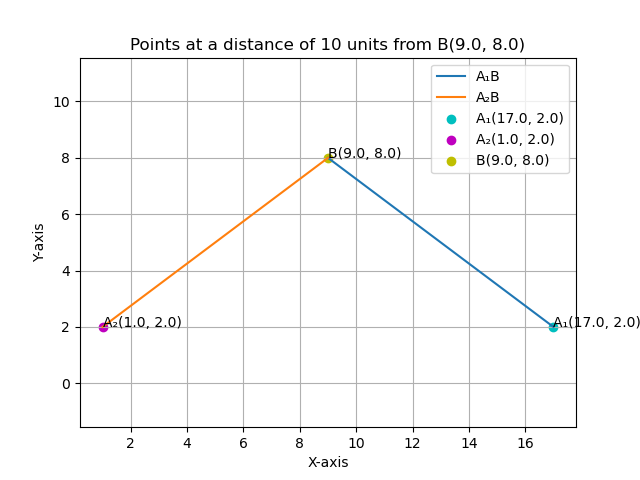
\includegraphics[width=0.8\linewidth]{figs/plot.png}
   	\caption{Plot of points $\vec{A_1}$ and $\vec{A_2}$ at a distance of $10$ units from $\vec{B}$}
\label{Plot}
\end{figure}
\end{document}
\end{document}
